\documentclass[aspectratio=1610]{beamer}

\usetheme{unnslides}
\usefonttheme{professionalfonts}

\usepackage[T2A]{fontenc}
\usepackage[utf8]{inputenc}
\inputencoding{utf8}
\usepackage{listings}
\usepackage{graphicx}
\usepackage{caption}
\usepackage{cmbright}
\usepackage{fontspec}
\usepackage{unicode-math}
\usepackage{amsfonts}
\usepackage{subfig}
\usepackage{tikz}

\captionsetup[subfigure]{labelformat=empty}
\captionsetup[figure]{labelformat=empty}

\setmainfont{CMU Sans Serif}
\setromanfont{CMU Sans Serif}
\setsansfont{CMU Sans Serif}

\setlength{\tabcolsep}{1pt}

\usepackage{polyglossia}
\setmainlanguage{russian}
%\setbeamertemplate{itemize item}{\color{black}$\blacktriangleright$}

\DeclareMathOperator*{\argmax}{arg\,max}
\DeclareMathOperator*{\argmin}{arg\,min}
\DeclareMathOperator{\sign}{sign}
\DeclareMathOperator{\re}{Re}

\graphicspath{ {../images/}{img/} }

%set pages numeration
\newcommand\numbered{\setbeamertemplate{footline}{%
  \vspace{-10em}
   \raisebox{5pt}{\makebox[\paperwidth]{%
     \hfill\makebox[10pt]{%
       \usebeamerfont{footline}\usebeamercolor[fg]{footline}
       \insertframenumber}}}}}
\newcommand\unnumbered{\setbeamertemplate{footline}{}}

\title{Параллельный алгоритм для получения равномерного приближения решений множества задач глобальной оптимизации с нелинейными ограничениями}
\author{\underline{\textbf{В.В.~Соврасов}} \and \textbf{К.А.~Баркалов}}
\institute{Нижегородский государственный университет им. Н.И. Лобачевского}
\date{}

\begin{document}
\numbered
{
\unnumbered
\begin{frame}[noframenumbering,plain]
\titlepage
\end{frame}
}

\begin{frame}
  \frametitle{Постановка задачи}
  \begin{columns}
    \begin{column}{0.5\textwidth}
      \begin{displaymath}
        \begin{array}{cr}\\
          \varphi(y^*)=\min\{\varphi(y):y\in D\}, \\
          D=\{y\in \mathbb{R}^N:a_i\leqslant y_i\leqslant{b_i}, \\ 1\leqslant{i}\leqslant{N},\:g_j(y)\leqslant 0, 1\leqslant j\leqslant m\}
        \end{array}
      \end{displaymath}
      \(\varphi(y),\:g_j(y)\) -- многоэкстремальные функции, удовлятворяющие условию Липшица:
      \begin{displaymath}
        \begin{array}{cr}\\
          |f(y_1)-f(y_2)|\leqslant L\Vert y_1-y_2\Vert,\\y_1,y_2\in \mathbb{R}^N:a_i\leqslant y_i\leqslant{b_i},
        \end{array}
      \end{displaymath}
      где \(L>0\) константа Липшица и \(||\cdot||\) обозначает \(l_2\) норму в пространстве \(\mathbb{R}^N\).
    \end{column}
    \begin{column}{0.5\textwidth}
      \centerline{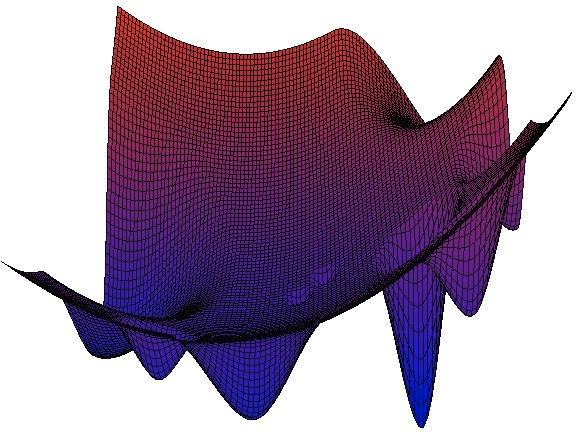
\includegraphics[width=0.9\textwidth]{img/gkls.png}}
    \end{column}
  \end{columns}
\end{frame}

\begin{frame}
  \frametitle{Постановка задачи}
  Далее будем интересоваться решением серии из \(q\) задач глобальной оптимизации с нелинейными ограничениями:
  \begin{displaymath}
    \min\left\{\varphi_1(y), y\in D_1 \right\}, \min\left\{\varphi_2(y), y\in D_2\right\},..., \min\left\{\varphi_q(y), y\in D_q\right\}.
  \end{displaymath}
  Подобные серии задач могут возникнуть, например, в следующих случаях:
  \begin{itemize}
    \item задача глобальной оптимизации с дискретным параметром;
    \item  решение задачи многокритериальной оптимизации методом свертки критериев.
  \end{itemize}
\textbf{Возможные методы решения}:
  \begin{itemize}
    \item решать каждую задачу независимо;
    \item разработать метод оптимизации, который решает все задачи из множества в совокупности, в каждый
    момент времени приоретизируюя одну из них.
  \end{itemize}
\end{frame}

\begin{frame}
  \frametitle{Редукция размерности}
  \begin{center}
  Кривая Пеано \(y(x)\) позволяет уменьшить размерность многомерного пространства до 1:
  \begin{gather}
    D_e=\lbrace y\in \mathbb{R}^N:-2^{-1}\leqslant y_i\leqslant 2^{-1},1\leqslant i\leqslant N\rbrace=\{y(x):0\leqslant x\leqslant 1\} \nonumber \\
    \min\{\varphi(y): y\in D\}=\min\{\varphi(y(x)): x\in [0,1]\} \nonumber
  \end{gather}
  \(y(x)\) является негладкой кривой, отображающей отрезок \([0,1]\) на гиперкуб \(D_e\).
  \begin{figure}[ht]
    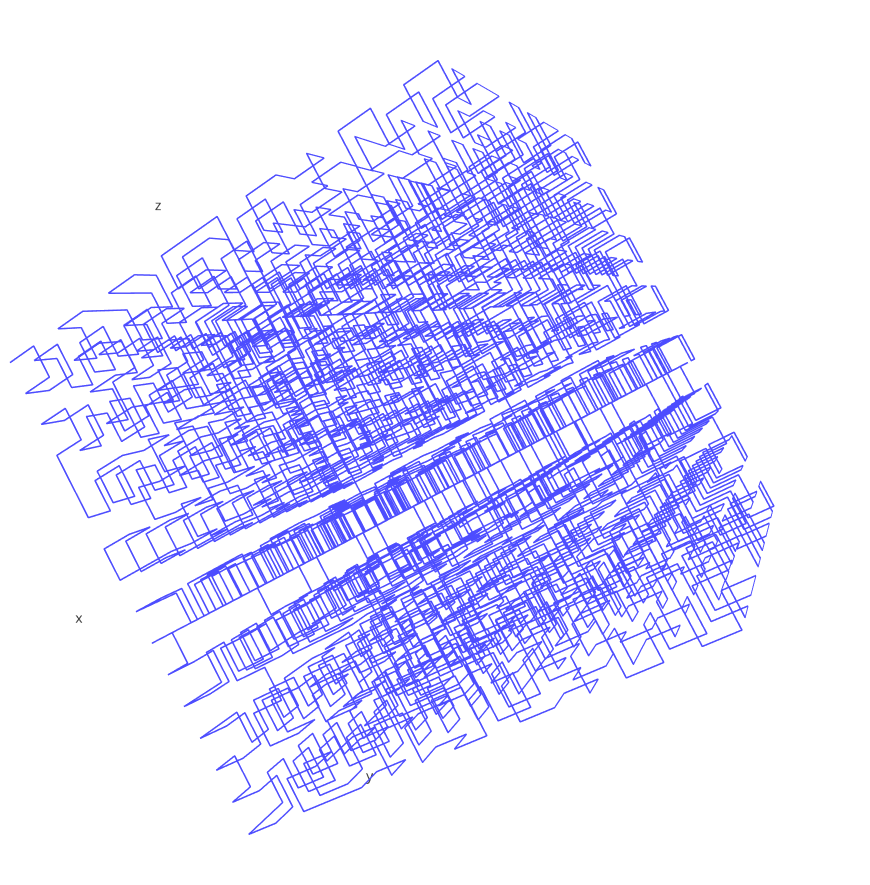
\includegraphics[width=.35\textwidth]{peano3d.png}
    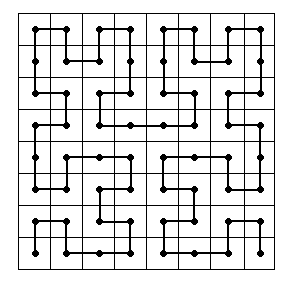
\includegraphics[width=.35\textwidth]{peano2d.png}
  \end{figure}
\end{center}
\end{frame}

\begin{frame}
  \frametitle{Алгоритм глобальной оптимизации}
  Метод оптимизации генерирует последовательность точек \(\{x_k:x_k\in[a,b]\}\) и состоит в выполнении следующих шагов:
  \begin{enumerate}
    \setlength{\itemindent}{.1in}
    \item[Шаг 1.] Упорядочить поисковую информацию (одномерные точки) по возрастанию.
    \item[Шаг 2.] Для каждого интервала \((x_{i-1}, x_i)\) вычислить величину \(R(i)\), называемую характеристикой.
    \item[Шаг 3.] Выбрать интервал \((x_{t-1}, x_{t})\) с наибольшей характеристикой и
    провести испытание (вычислить органичения и целевую функцию) в точке \(x^{k+1}\), выбранной с помощью решающего правила \(d\):
    \begin{displaymath}
      x^{k+1}=d(t)\in (x_{t-1}, x_{t})
    \end{displaymath}
    \item[Шаг 4.] Если \(x_{t}-x_{t-1}<\varepsilon\), остановить метод.
  \end{enumerate}
  \textit{\footnotesize	{Детальное описание метода: Strongin R.G., Sergeyev Ya.D.: Global optimization with non-convex constraints. Sequential and parallel algorithms (2000), Chapter 7}}
\end{frame}

\begin{frame}
  \frametitle{Алгоритм, решающий множество задач}
  Модификация метода для решения множества задач:
  \begin{itemize}
    \item Создать \(q\) копий характеристического АГО.
    \item Использовать \(q\) синхронно работающих копий АГО с тем лишь отличием, что на шаге 3 при выборе
    интервала с наилучшей характеристикой, выбор будет осуществляться из всех интервалов, которые
    породили на данный момент \(q\) копий АГО.\
    \item Если наибольшая характеристика соответствует
    задаче \(i\), то выполняется шаг 3 в копии метода с номером \(i\), а остальные копии метода простаивают.
    \item Для реализации параллельности в предыдущем пункте можно выбрать \(p\) характеристик и провести
    испытания в \(p\) задачах одновременно.
  \end{itemize}
  Чтобы приведённая схема работала, требуется \textbf{сравнимость характеристик интервалов в разных задачах}.
\end{frame}

\begin{frame}
  \frametitle{Индексная схема учёта ограничений}
  Вместо исходной задачи рассмотрим следующую задачу без функциональных ограничений:
  \begin{displaymath}
    \begin{array}{lr}
      \psi (x^{*})=\min_{x\in [0;1]}\psi (x), \\
      \psi (x)={\begin{cases}g_{\nu }(x)/H_{\nu }&\nu <M\\(g_{M}(x)-g_{M}^{*})/H_{M}&\nu =M\end{cases}}
    \end{array}
  \end{displaymath}
  где при \(\nu=m+1\;g_\nu(x)=\varphi(x)\).

  При использовании индексной схемы характеристики определяются следующим образом:
  \begin{displaymath}
    R(i)={\begin{cases}\Delta _{i}+{\frac {(z_{i}-z_{i-1})^{2}}{(r_{\nu }\mu _{\nu })^{2}\Delta _{i}}}-2{\frac {z_{i}+z_{i-1}-2z_{\nu }^{*}}{r_{\nu }\mu _{\nu }}}&\nu =\nu (x_{i})=\nu (x_{i-1})\\2\Delta _{i}-4{\frac {z_{i-1}-z_{\nu }^{*}}{r_{\nu }\mu _{\nu }}}&\nu =\nu (x_{i-1})>\nu (x_{i})\\2\Delta _{i}-4{\frac {z_{i}-z_{\nu }^{*}}{r_{\nu }\mu _{\nu }}}&\nu =\nu (x_{i})>\nu (x_{i-1})\end{cases}}
  \end{displaymath}
  где \(z_i=\psi(x_i)\). Можно показать, что при использовании таких характеристик метод будет выбирать интервалы из всех \(q\) задач, тем самым решая их все, а не только некоторое подмножество задач.
\end{frame}

\begin{frame}
  \frametitle{Пример решения многокритериальной задачи}
  Рассматриваемая задача:
  \begin{displaymath}
    \begin{array}{l}
        Minimize \left \{
        \begin{array}{l}
          f_1(y) = 4 y_1^2 + 4 y_2^2 \\
          f_2(y) = (y_1-5)^2 + (y_2-5)^2 \\
        \end{array}
        \right .
        y_1\in [-1;2],y_2\in [-2;1]
        \\s.t.
        \\
        \left \{
        \begin{array}{l}
          g_1(y) = (y_1 - 5)^2 + y_2^2 - 25 \leqslant 0 \\
          g_2(y) = -(y_1 - 8)^2 - (y_2 + 3)^2 + 7.7 \leqslant 0\\
        \end{array}
        \right .
    \end{array}
  \end{displaymath}
  После использования свёртки Гермейера для скаляризации задача примет вид:
  \begin{displaymath}
    \varphi(y^*(\lambda_1,\lambda_2))=\min_{y\in D}\max\{\lambda_1 f_1(y), \lambda_2 f_2(y)\};\lambda_1,\lambda_2\in[0,1],\: \lambda_1+\lambda_2=1
\end{displaymath}
Для численного построения множества Парето выберем
100 наборов коэффициентов \((\lambda_1,\lambda_2)\) таких, что
\(\lambda_1^i=i h,\: \lambda_2^i=1-\lambda_1^i,\: h=10^{-2},i=\overline{1, 100}\).
\end{frame}

\begin{frame}
  \frametitle{Пример решения многокритериальной задачи}
  \vspace*{-1.0cm}
  \begin{displaymath}
    \begin{array}{cr}\\
      SP(S)=\sqrt{\frac{1}{|S|-1} \sum_{i=1}^{|S|} (\overline{d}-d_i)^2},\:\overline{d}=mean\{d_i\}, \\
      d_i=\min_{s_i,s_j\in S:s_i\ne s_j}||F(s_i)-F(s_j)||_1,\: F=(f_1,f_2)
    \end{array}
  \end{displaymath}

  \begin{figure}[ht]
      \centering
      \vspace*{-0.5cm}
      \subfloat[Раздельное решение задач, \(SP_{single}=0.984\)]{
      \label{fig:mco_pareto_1} {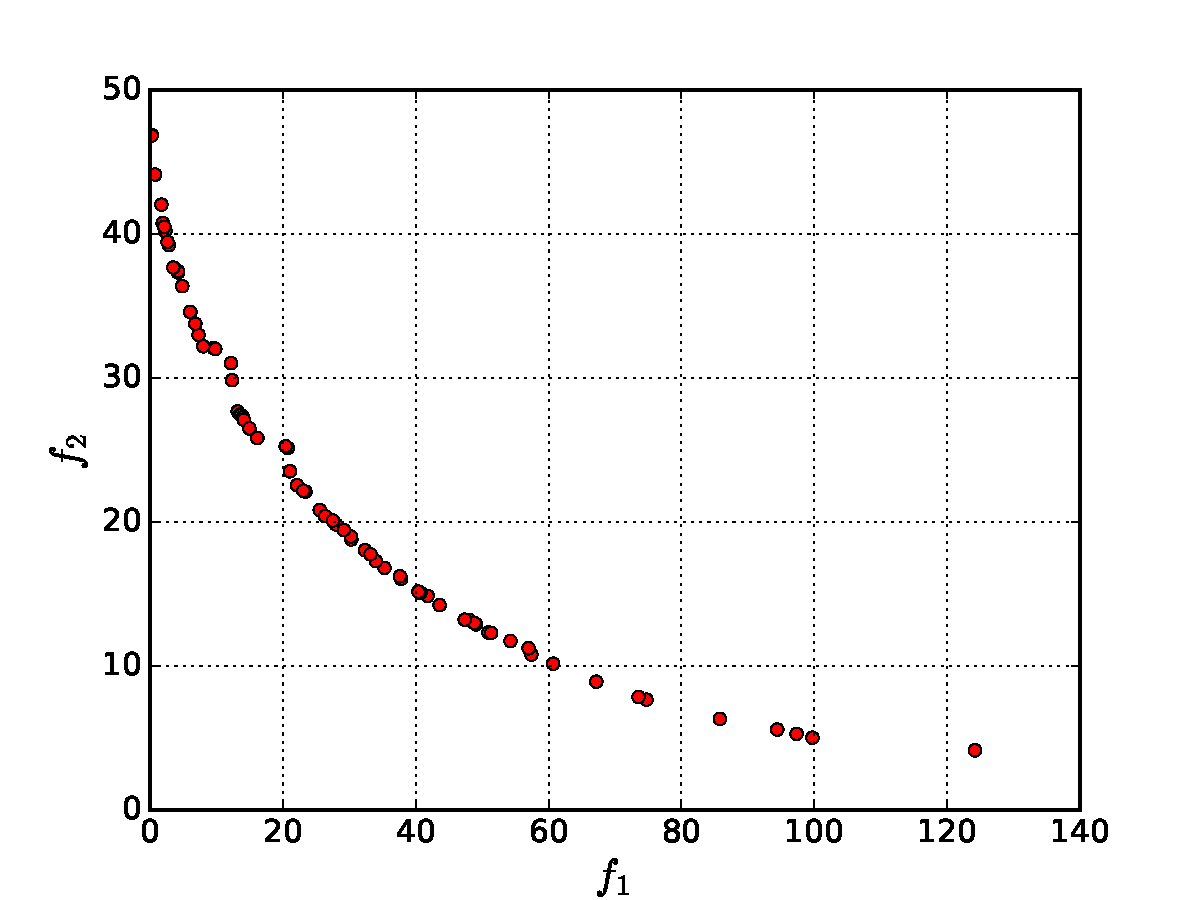
\includegraphics[width=.5\textwidth]{single_mco.pdf}}}
      \subfloat[Решение множества задач, \(SP_{multi}=0.749\)]{
      \label{fig:mco_pareto_2} {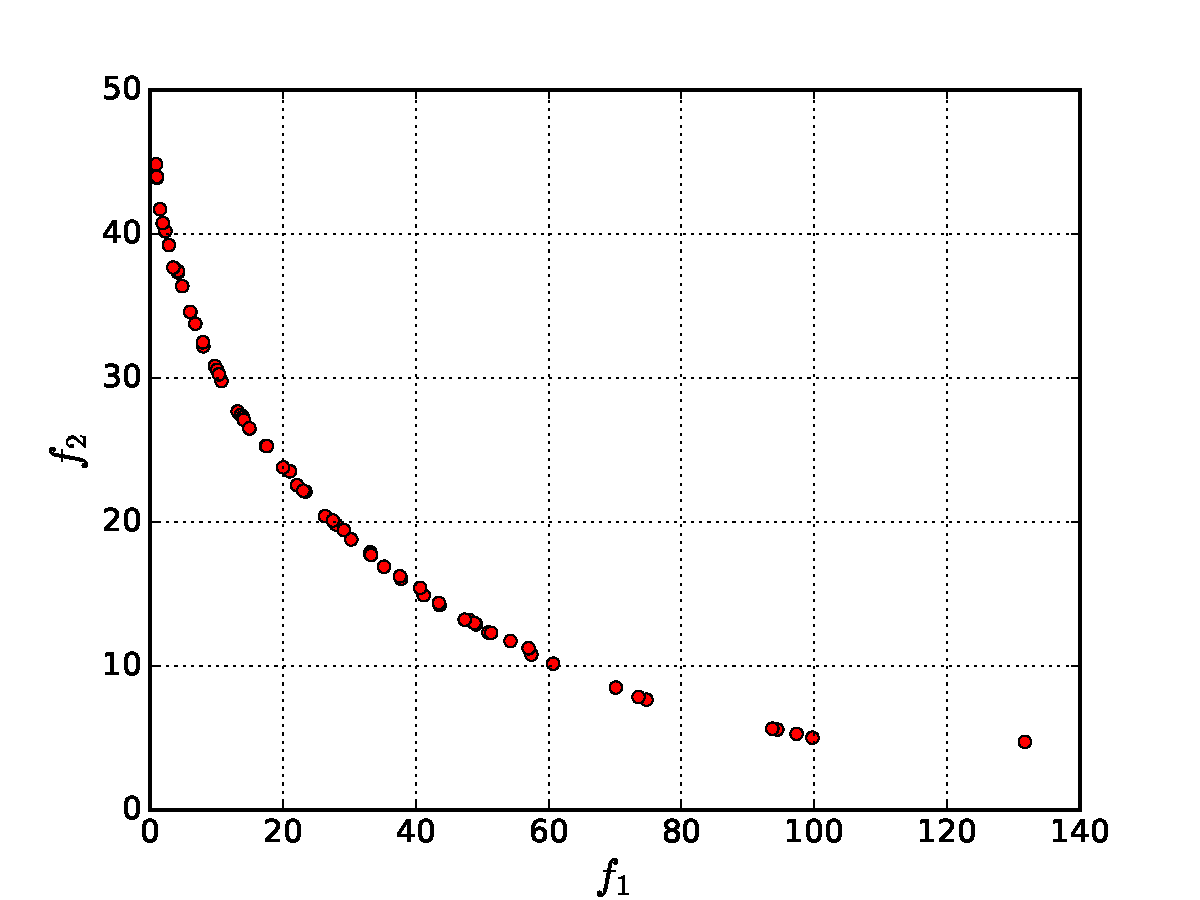
\includegraphics[width=.5\textwidth]{multi_mco.pdf}}}
      \caption{Численные оценки множества Парето, полученные после 2500 испытаний}
      \label{fig:mco_pareto}
  \end{figure}
\end{frame}

\begin{frame}
  \frametitle{Тестовые многомерные задачи с ограничениями}
  \begin{columns}
    \begin{column}{0.5\textwidth}
      Тестовые наборы были получены с помощью системы GCGen, позволяющей
      сторить многомерные задачи с ограничениями из заданных функций, и нескольких
      известных генераторов тестовых задач (GKLS, \(F_{GR}\)).
      Характеристики каждого из сгенерированных наборов задач:
      \begin{itemize}
        \item \(q\)=100;
        \item Размерность 2 или 3;
        \item Базовые функции только GKLS или \(F_{GR}\), или их комбинация;
        \item Количество ограничений: 2.
      \end{itemize}
    \end{column}
    \begin{column}{0.5\textwidth}
      \centerline{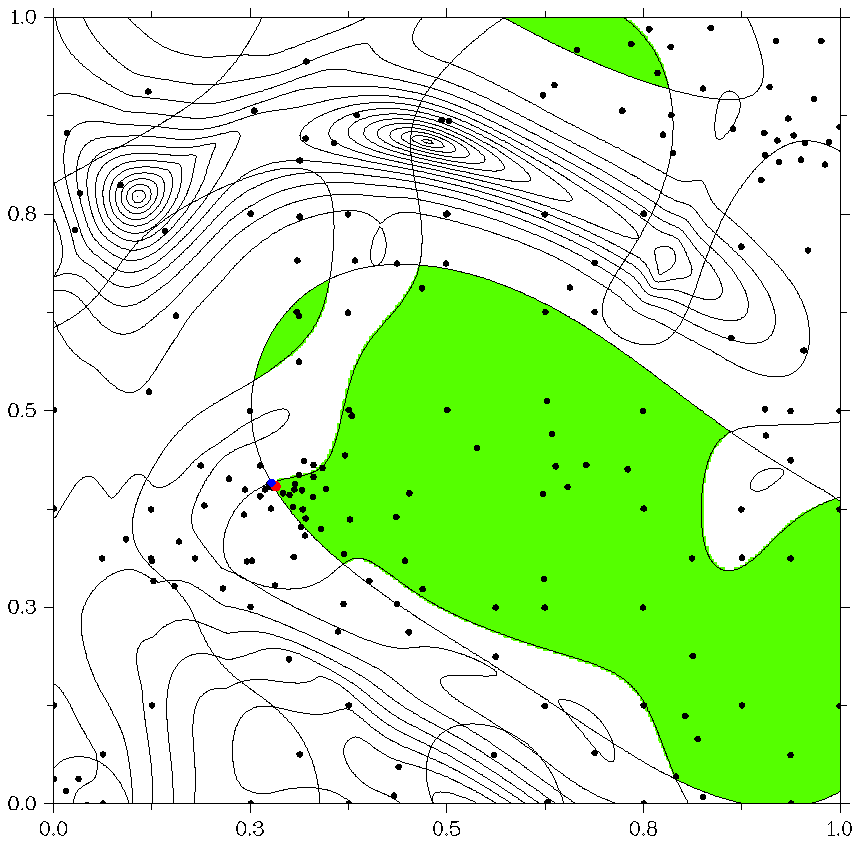
\includegraphics[width=0.9\textwidth]{4.png}}
    \end{column}
  \end{columns}
  \footnotesize{Система GCGen доступна по ссылке \textit{https://github.com/UNN-ITMM-Software/GCGen}}
\end{frame}

\begin{frame}
  \frametitle{Программное и техническое обеспечение}
  \begin{center}
    Реализация параллельного метода была выполнена на языке C++ с использованием технологии OpenMP
    для распареллеливания процесса проведения испытаний на общей памяти.

    Все вычислительные
    эксперименты проведены на машине со следующей конфигурацией: Intel Core i7-7800X (6 cores) CPU, 64GB RAM, Unubtu 16.04 ОS, GCC 5.5 compiler.
  \end{center}
\end{frame}

\begin{frame}
  \frametitle{Результаты экспериментов на наборах синтетических задач}
  \begin{figure}[ht]
    \vspace*{-0.5cm}
      \centering
      \subfloat[\(D_{max}\)]{
      \label{fig:max_dev} {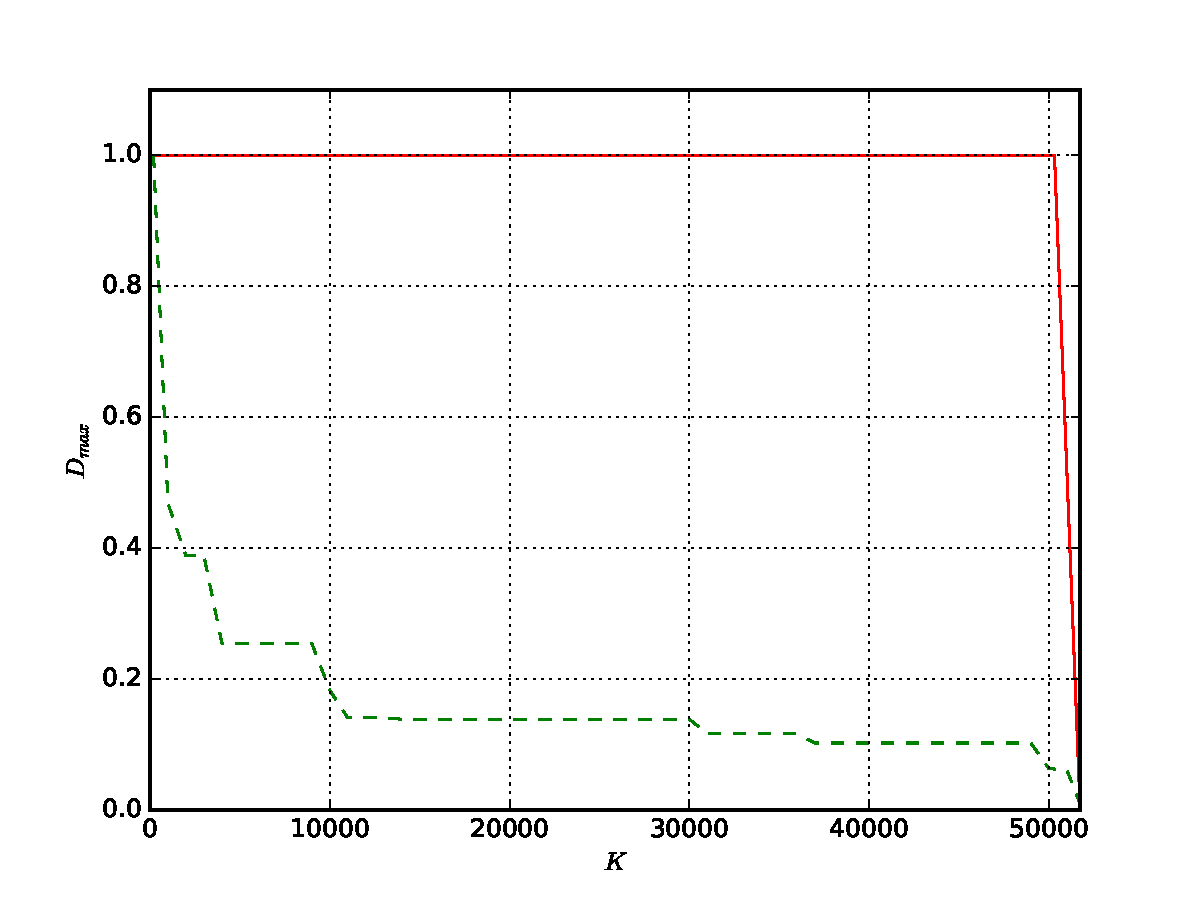
\includegraphics[width=.5\textwidth]{mixed_2d_max.pdf}}}
      \subfloat[\(D_{avg}\)]{
      \label{fig:avg_dev} {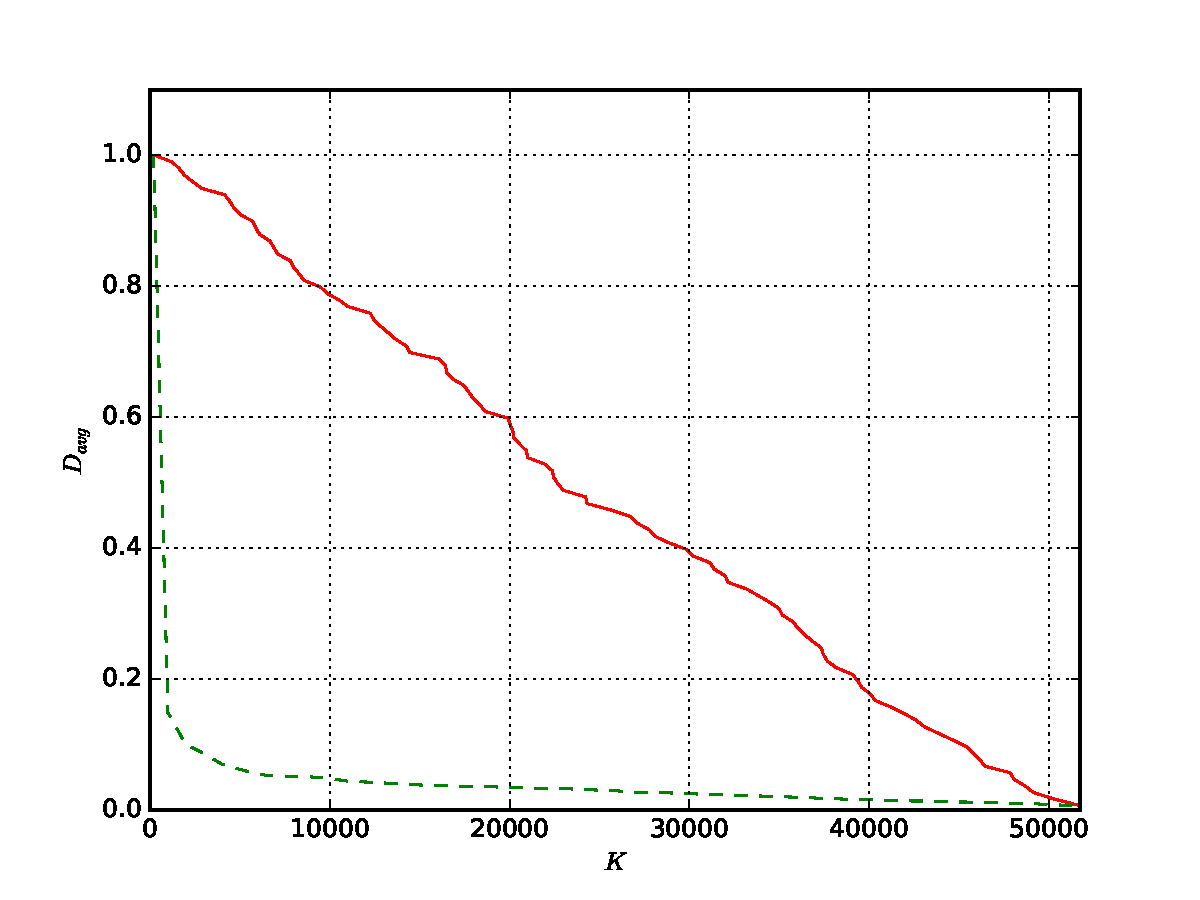
\includegraphics[width=.5\textwidth]{mixed_2d_avg.pdf}}}
      \caption{Динамика величин средней по задачам и максимальной точности в процессе решения множества двухмерных задач,
      порождённых двумя разными генераторами GKLS и \(F_{GR}\)}
      \label{fig:devs_mixed}
  \end{figure}
\end{frame}

\begin{frame}
  \frametitle{Результаты экспериментов на наборах синтетических задач}
  \begin{table}
    \centering
    \begin{tabular}{c|c|c|c|c|c}
      %\cline{1-8}\noalign{\smallskip}
      Класс задач & \textit{p} & Количество итераций & Время, с & \(S_i\) & \(S_t\)   \\
      %s\noalign{\smallskip} \cline{4-5} \cline{7-8}  \noalign{\smallskip}
      \hline
      GKLS \& \(F_{GR}\)-based \
        & 1 & 51434 & 90.20 & -    & - \\
        & 2 & 25698 & 56.96 & 2.00 & 1.58 \\
        & 4 & 13015 & 36.67 & 3.95 & 2.46 \\
        & 6 & 8332  & 26.85 & 6.17 & 3.36 \\
      \hline
      GKLS-based 2d \
        & 1 & 59066 & 97.53 & -    & - \\
        & 2 & 29060 & 60.56 & 2.04 & 1.61 \\
        & 4 & 14266 & 38.92 & 4.14 & 2.51 \\
        & 6 & 9436  & 29.53 & 6.26 & 3.30 \\
      \hline
      GKLS-based 3d \
        & 1 & 782544 & 1117.55 & -    & - \\
        & 2 & 397565 & 752.92  & 1.97 & 1.48 \\
        & 4 & 208073 & 526.67  & 3.76 & 2.12 \\
        & 6 & 142089 & 445.45  & 5.50 & 2.51 \\
      \hline
    \end{tabular}
  \end{table}
\end{frame}

\begin{frame}
  \frametitle{Заключение}
  В ходе работы были достигнуты следующие результаты:
    \begin{itemize}
      \item реализована поддержка нелинейных ограничений в алгоритме, решающeм
      множество задач глобальной оптимизации;
      \item проведены численные эксперименты, демонстрирующие преимущество рассматриваемого подхода в скорости сходимости на всём множестве задач в среднем над решением задач по отдельности;
      \item показана эффективность совместного решения множества задач на примере решения многокритериальной задачи с нелинейными ограничениями.
    \end{itemize}

    В ходе дальнейшей работы планируется:
    \begin{itemize}
      \item улучшить текущую реализацию алгоритма, сократив расходы на содержание поисковой информации для множества задач и тем самым улучшив
      показатели параллельного ускорения по времени;
      \item реализовать версию рассматриваемого алгоритма, работающего на распределенной памяти.
    \end{itemize}
\end{frame}

{
\unnumbered
\begin{frame}{{}}
  \frametitle{Q\&A}
  \begin{center}
    \Large{Контакты:}
\vspace{0.5cm}

    sovrasov.vlad@gmail.com

    https://github.com/sovrasov
  \end{center}
\end{frame}
}
\end{document}
